\section{Durchführung}
Die Schaltung des Versuchs ist in Abbildung \ref{fig:Schaltung} dargestellt.
\begin{figure}[H]
  \centering
  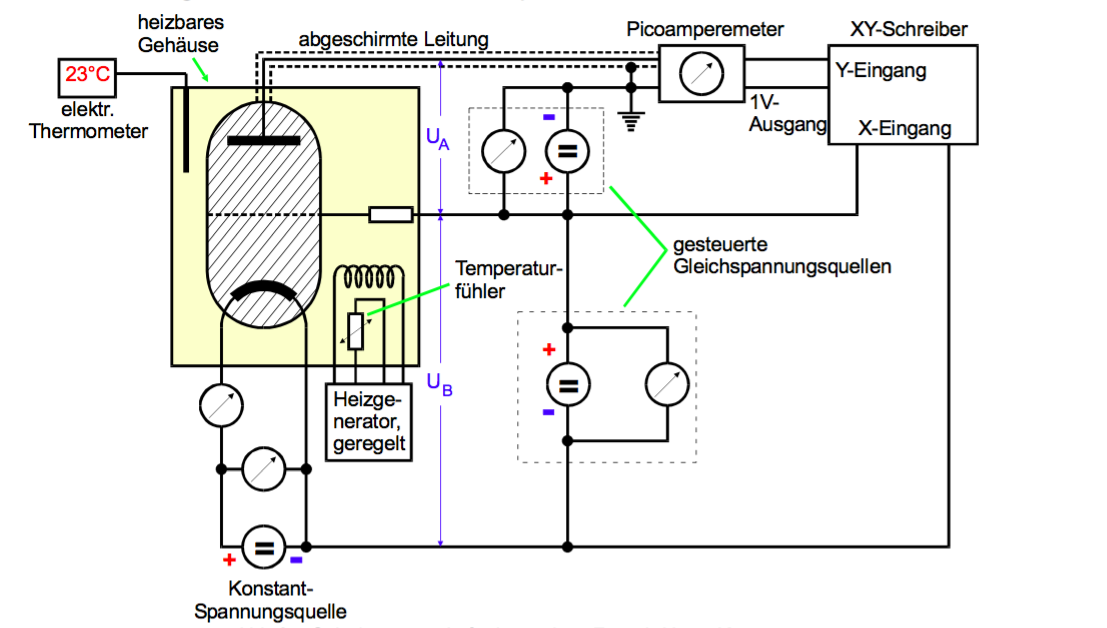
\includegraphics[height=5cm]{Schaltung.png}
  \caption{Versuchsaufbau und Schaltung \cite{skript}.}
  \label{fig:Schaltung}
\end{figure}
Die Aufzeichnung der Messergebnisse erfolgt über einen XY-Schreiber, welcher vor
Versuchsbeginn zuerst noch justiert werden muss. Dazu wird das Millimeterpapier eingelegt
und zunächst mit den Knöpfen "Zero" der Nullpunkt in die linke untere Ecke gelegt.
Anschließend wird die Empfindlichkeit eingestellt, wobei in einem Unempfindlichen Bereich
angefangen wird und dann langsam hochgedreht wird, um den Antriebsmotor nicht zu überlasten.
Liegt die Maximalspannung der Messreihe für den X-Eingang schlussendlich am rechten Rand,
muss die x-Achse nun noch kalibriert werden, indem der gesamte Bereich ohne Y-Ausschlag einmal
abgefahren wird und einige Zwischenpunkte makiert werden. \\
Zur Messung der integralen Energieverteilung der Elektronen wird eine konstante
Beschleunigungsspannung von $\text{U}_B = \SI{11}{\volt}$ eingestellt. Dann wird die
Bremsspannung $\text{U}_A$ mit dem X-Eingang und die proportionale Spannung zum Auffängerstrom $\text{I}_A$
mit dem Y-Eingang des XY-Schreibers verbunden. Die Bremsspannung wird dann zeitproportional
zwischen 0-1o$\si{\volt}$ variiert und der entsprechende Auffängerstrom gemessen.
Eine Messung wird dabei bei etwa 20°C durchgeführt und eine im Bereich von etwa
140°C bis 160°C. \\
Für die Aufnahme der Franck-Hertz Kurven wird $\text{U}_A$ konstant auf etwa $\SI{1}{\volt}$
eingestellt. Der X-Eingang wird mit der Beschleunigungsspannung $\text{U}_B$ verbunden
und der Y-Eingang erneut mit der Spannung proportional zu $\text{I}_A$. Nach erneuter
Justierung wird nun die Beschleunigungsspannung zwischen 0 und 60$\si{\volt}$ variiert und dabei
der zugehörige Auffängerstrom gemessen. Dabei werden solange Franck-Hertz
Kurven im Temperaturbereich zwischen 160°C und 200°C aufgezeichnet, bis eine zur
Auswertung brauchbare gefunden wird. \\
Anschließend wird noch die Ionisationsenergie von Hg gemessen, indem $\text{U}_A = - \SI{30}{\volt}$ eingestellt
wird und bei einer Temperatur zwischen 100°C und 110°C erneut der Auffängerstrom in Abhängigkeit
der Beschleunigungsspannung aufgezeichnet wird.
